\documentclass{book}
\usepackage{graphicx}
\usepackage{amsmath}

\newtheorem{definition}{Definition}

\begin{document}
    \chapter{Fundamentals}
    \begin{definition}[Pitch]
        Pitch is the property of the sound which allows a relative ordering of perceived sounds on a frequency-related scale.
    \end{definition}
    On a keyboard, pitch goes up to the right of the keyboard, while it goes down on the left.

    Pitches are expressed through \textbf{notes}. There are 7 note names, which are repeated in \textbf{octave registers}, identified by the bottom number.
    $$A_3 B_3 \underbrace{C_4 D_4 E_4 F_4 G_4 A_4 B_4}_{\text{Octave register 4}} C_5 D_5$$

    \begin{figure}
        \begin{center}
            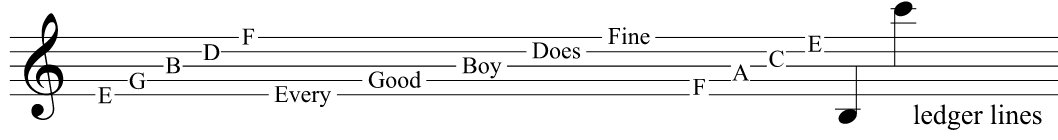
\includegraphics[width=0.8\textwidth]{img/treble}
            \caption{Treble clef}
            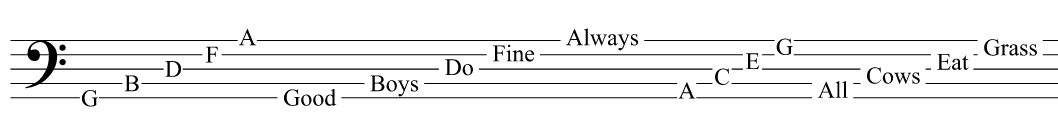
\includegraphics[width=0.8\textwidth]{img/bass}
            \caption{Bass clef}
        \end{center}
    \end{figure}
\end{document}